%%
%% Author: dariochinelli
%% 2021-03-27
%%

\section{Approfondimento sulla statistica classica di Maxwell-Boltzmann}

Riprendiamo la legge di distribuzione
\begin{equation}
n_s = \frac{N}{Z} g_s e^{ - \beta E_s }
\label{leg_dist_ns}
\end{equation}
legata alla funzione di partizione
\begin{equation}
Z = \sum_s e^{ - \beta E_s }
\label{fun_part}
\end{equation}
Dove i moltiplicatori di Lagrange $\alpha$ e $\beta$ sono legati al numero di particelle $N$ e all'energia $U$.
Il valore medio di una certa proprietà $F_{avg}$ dipendente dall'energia $E_s$
\begin{equation}
\begin{split}
F_{avg} = \langle F \rangle & =  \frac{1}{N} \sum_s n_s F(E_s) \\
& = \frac{1}{Z} \sum_s g_s F(E_s) e^{- \beta E_s}
\end{split}
\end{equation}

\subsection{Temperatura}
Classicamente la temperatura è stata introdotta per descrivere un'esperienza sensoriale, non statistica...
Facendo l'analisi dimensionale delle equazioni di $n_s$ e $Z$ si deriva che il fattore $\beta$ deve essere espresso in $1/joule$
affinché siano soddisfatte.

Se nell'espressione dell'energia sostituisco i valori $n_s$ della \ref{leg_dist_ns}, trovo
\begin{equation}
\begin{split}
U = n_1 E_1 + n_2 E_2 + ... & = \frac{ N}{Z } \Bigl(  g_1 E_1 e^{ -\beta E_1 } + g_2 E_2 e^{ -\beta E_2 } + ... \Bigr) \\
& = \frac{ N}{Z } \Bigl(  \sum_s g_s E_s e^{ -\beta E_s }  \Bigr)
\end{split}
\end{equation}
usando la definizione di funzione di partizione \ref{fun_part} si trova
\begin{equation}
\begin{split}
U &= - \frac{ N}{Z } \frac{ d}{d\beta }  \Bigl(  \sum_s g_s E_s e^{ -\beta E_s }  \Bigr) \\
& = - \frac{ N}{Z } \frac{ d Z}{d\beta } \\
& = - N \frac{ d}{d\beta }(\ln Z)
\label{energia_totale}
\end{split}
\end{equation}
L'energia media di ogni particella del sistema sarà
\begin{equation}
E_{avg} =  \langle E \rangle = \frac{ U}{N } = - \frac{ d}{d\beta } (\ln Z)
\label{energia_media}
\end{equation}
Da cui si vede che dato un certo sistema fisico descritto da valori $E_s$ e $g_s$ ben precisi, la funzione di partizione \ref{fun_part}, l'energia totale \ref{energia_totale} e l'energia media \ref{energia_media} risultano essere tutte funzioni di $\beta$;
significa che posso utilizzare $\beta$ per caratterizzare tutte queste funzioni.
Si trova però più conveniente introdurre un'altra variabile, funzione di $\beta$, ovvero la \textit{temperatura}, definita come:
\begin{equation}
\begin{split}
& k_B T = \frac{1}{\beta} \\
& k_B = \SI{1.3805e-23}{j / K} = \SI{8.6178e-5}{eV / K} \quad\quad \mbox{costante di Boltzmann}
\end{split}
\end{equation}
si noti che la grandezza $k_B T$ è un'\textit{energia termica}, ad esempio ponendoci a temperatura ambiente con $T_{amb}=\SI{300}{K}$ l'energia termica equivale a $k_B T_{amb} = \SI{0.0258}{eV} \simeq \SI{26}{m eV} $. \\
\textbf{NB:} Questa definizione di temperatura è valida solo per sistemi di particelle all'\textit{equilibrio statistico}. \\
Posso allora riscrivere le relazioni precedenti 
\begin{equation}
Z = \sum_s g_s e^{ - \frac{E_s}{k_B T} }
\end{equation}
\begin{equation}
n_s = \frac{N}{Z} g_s e^{ - \frac{E_s}{k_B T} }
\label{funz_dist_ns_T}
\end{equation}
il differenziale di $\beta$ è
\begin{equation}
d \beta = - \frac{d T}{k T^2}
\end{equation}
allora la relazione per l'energia totale è
\begin{equation}
U = k N T^2 \frac{d}{dT} (\ln Z)
\end{equation}
e l'energia media per particella è
\begin{equation}
\langle E \rangle = \frac{U}{N} = k T^2 \frac{d}{dT} (\ln Z)
\label{energia_cinetica_media}
\end{equation}
Il valore medio di una certa grandezza $F$ dipendente dall'energia è
\begin{equation}
\langle F \rangle = \frac{1}{Z} \sum_s g_s F(E_s) e^{ -\frac{E_s}{k_B T} }
\end{equation}
quindi la media di una funzione dipendente dall'energia è funzione della temperatura.
L'equazione \ref{funz_dist_ns_T} permette di capire che ad una certa temperatura $T$ fissata, l'occupazione di livelli di energia disponibili diminuisce all'aumentare della loro energia, si vanno ad occupare i livelli con energia sempre più elevata: 
quello che succede è che l'aumento di temperatura equivale all'aumento dell'energia totale delle particelle.
\begin{figure}[h]
\centering
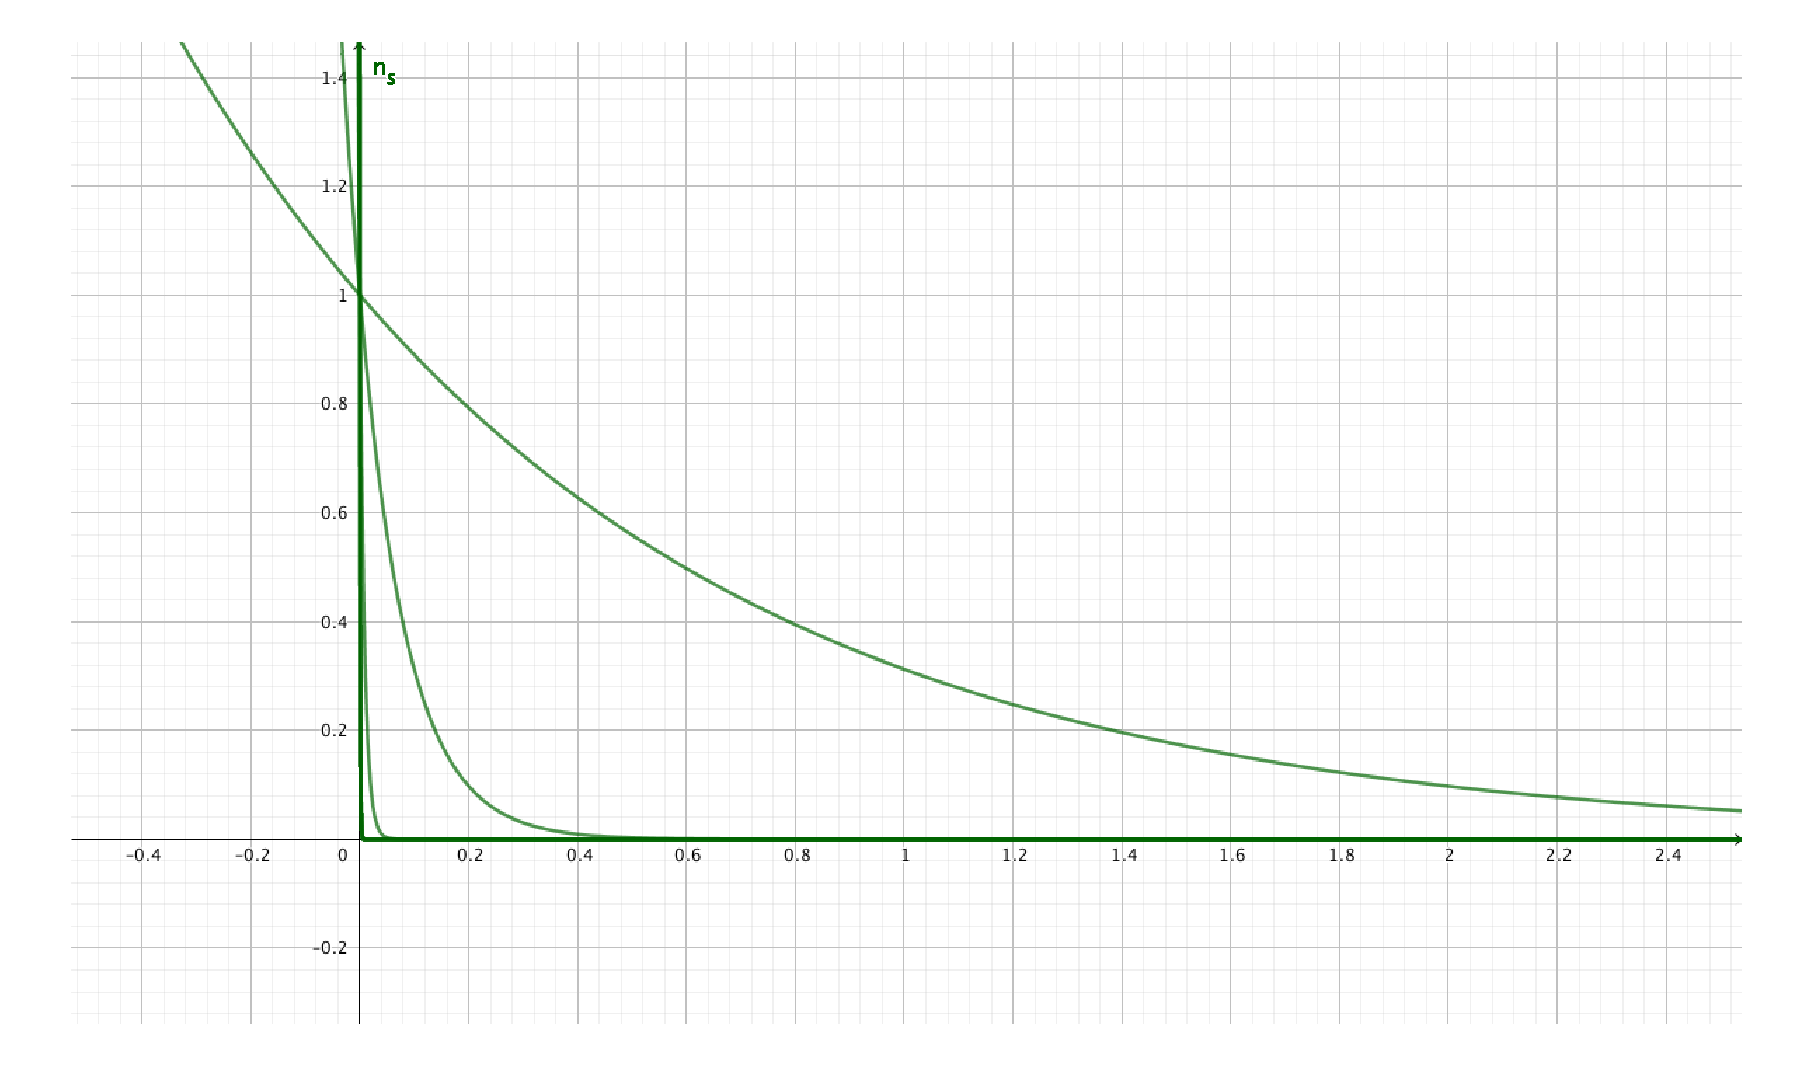
\includegraphics[scale=0.35]{/livelli_occupati}
\caption{Grafico qualitativo della funzione di partizione \ref{funz_dist_ns_T} per diverse temperature }
\end{figure}

Il rapporto tra il numero di occupazione tra due stati generici $\frac{n_i}{n_j}$ è 
\begin{equation}
\begin{split}
\frac{n_i}{n_j} & = \frac{g_i}{g_j} e^{ - \frac{(E_i - E_j)}{k_B T} } \\
& = \frac{g_i}{g_j} e^{ - \frac{- \Delta E}{k_B T} }
\end{split}
\end{equation}
permette di capire che due livelli sono confrontabili se $\Delta E \ll k_B T$ e l'esponenziale tende a 1.


\subsection{La funzione densità degli stati}
si può ricavare dalla fisica classica, ottenendo il seguente risultato
\begin{equation} 
g(E) = \frac{4 \pi V (2m^3)^{ \frac{1}{2} }}{h^3} E^{ \frac{1}{2} }
\label{dens_stati}
\end{equation}
Innanzitutto definire uno \textit{stato} in fisica classica significa esprimere, in un certo istante, le coordinate ed il momento di una particella (quindi $p$ e $q$). 
Questi stati sono quindi punti nello spazio delle fasi e determinare la funzione densità degli stati in fisica classica significa determinare, o contare, i punti nello spazio delle fasi corrispondente ad un certo intervallo di energia.
Posso postulare che il numero di stati sia proporzionale al \textit{volume} dello spazio delle fasi, anche se in fisica classica sarebbe un numero infinito.
Vediamo di seguito due esempi per ricavare la funzione densità degli stati: nel caso di particella libera e nel caso di oscillatore armonico.

\paragraph{Caso articella libera}
Assumiamo che il valore minimo dell'energia sia $zero$ e scrivo l'energia della particella libera
\begin{equation}
E = \frac{p^2}{2m} 
\end{equation}
Allora il numero di stati possibili in funzione dell'energia nell'intervallo $[0, E]$ sarà \underline{proporzionale} a
\begin{equation}
N(E) \propto 4 \pi \int p^2 dp d^3q = 4 \pi V \int_{\frac{p^2}{2m} \le E } p^2 dp
\end{equation}
in cui $V$ è il volume
\begin{equation}
V = \int d^3 q
\end{equation}
\begin{equation}
\begin{split}
pongo &\quad\quad x = \frac{p}{\sqrt{2m E}} \\
con condizione &\quad\quad \frac{p^2}{2m} \le E \\
\Rightarrow\quad ottengo &\quad\quad x^2 \le 1
\end{split}
\end{equation}
sostituendo nell'integrale
\begin{equation}
N(E) \propto 4\pi V \int_{x^2 \le 1} x^2 dx (2mE)^{ \frac{3}{2} }
\end{equation}
la condizione $x^2 \le 1$ significa integrare tra $[0, 1]$ quindi
\begin{equation}
N(E) \propto 4\pi V \Bigl[  \frac{x^3}{3}  \Bigr]_0^1 (2mE)^{ \frac{3}{2} } = \frac{4\pi}{3} V (2m)^{ \frac{3}{2} }(E)^{ \frac{3}{2} }
\end{equation}
quindi per calcolare il numero di stati tra $E$ e $E + dE$ derivo rispetto all'energia $E$
\begin{equation}
\begin{split}
g(E) dE & = \frac{d N(E)}{dE} dE \\
g(E) dE & \propto \frac{4\pi}{3} V (2mE)^{\frac{3}{2}} \frac{d (E^{ \frac{3}{2} }) }{dE}  dE \\
\Rightarrow\quad g(E) dE & \propto 4\pi V (2m^3)^{\frac{1}{2}} E^{ \frac{1}{2} }  dE
\end{split}
\end{equation}
La differenza rispetto alla formula \ref{dens_stati}, scritta sopra e ricavata precedentemente, sta solo nel fattore $h^3$ a denominatore.
Ciò significa che ogni stato delle fasi non può essere rappresentato da un punto ma deve avere un volume definito, tale volume equivale a
\begin{equation}
\Delta x \Delta p_x \approx h
\end{equation}
per ogni dimensione, quindi elevandolo alla terza si ottiene il fattore di conversione che permette di sostituire il \textit{proporzionale} con un \textit{uguale}.

\paragraph{Caso oscillatore unidimensionale}
L'energia in questo caso sarà
\begin{equation}
\begin{split}
E & = \frac{p^2}{2m} + \frac{1}{2} K q^2 \\
& K \quad \mbox{costante elastica}
\end{split}
\end{equation}
come prima cerco il numero di stati possibili in funzione dell'energia nell'intervallo $[0, E]$ sarà \underline{proporzionale} a
\begin{equation}
N(E) \propto \int_{\frac{p^2}{2m E} + \frac{K q^2}{2E} \le 1 } dp dq
\end{equation}
\begin{equation}
\begin{split}
pongo &\quad\quad x = \frac{p}{\sqrt{2m E}} \quad\quad y = \frac{q}{\sqrt{2E}} \sqrt{K}  \\
con condizione &\quad\quad  \frac{p^2}{2m} + \frac{1}{2} K q^2  \le E 
\quad\Rightarrow\quad \frac{p^2}{2mE} + \frac{K q^2}{2E}   \le 1 \\
\Rightarrow\quad ottengo &\quad\quad x^2 + y^2 \le 1
\end{split}
\end{equation}
riscrivendo l'integrale nelle nuove variabili $x, y$ ottengo
\begin{equation}
N(E) \propto \int_{x^2 + y^2 \le 1} 2E\sqrt{\frac{m}{k}} dx dy
\end{equation}
in cui si integra su una circonferenza.
La relazione fondamentale per un oscillatore generico è
\begin{equation}
\omega = \sqrt{\frac{K}{m}} = 2\pi \nu
\end{equation}
da cui risulta che
\begin{equation}
N(E) \propto \frac{E}{\nu}
\end{equation}
e quindi
\begin{equation}
g(E)dE = \frac{dN(E)}{dE} dE \propto \frac{1}{\nu} dE
\label{gE_costante}
\end{equation}
per un oscillatore armonico la distribuzione degli stati non dipende dall'energia.

\paragraph{Rispetto al corpo nero} avevamo introdotto la statistica classica di Maxwell Boltzmann 
\begin{equation}
P(\varepsilon) d\varepsilon = \frac{1}{k_BT} e^{ -\frac{\varepsilon}{k_BT} } d\varepsilon
\end{equation}
definendo la probabilità $P(\varepsilon)$ di trovare una certa quantità di un sistema con energia nell'intervallo $d\varepsilon$.
Tali entità erano le \textit{onde stazionarie} all'interno della cavità di corpo nero, che sono effettivamente l'analogo di un oscillatore armonico
Tale statistica è vera quando il numero degli stati di energia non dipende da $\varepsilon$, fatto verificato poco sopra.
L'energia media $\bar \varepsilon$ delle onde stazionarie era stata scritta nella forma \ref{energia_media_blackbody}
\begin{equation}
\bar\varepsilon=\frac{\int_{0}^{\infty} \varepsilon P(\varepsilon)\,d\varepsilon}{\int_{0}^{\infty} P(\varepsilon)\,d\varepsilon} = \frac{\int_{0}^{\infty} \varepsilon \frac{ e^{ - \frac{\varepsilon}{kT } } }{kT } d\varepsilon}{\int_{0}^{\infty} \frac{ e^{ - \frac{\varepsilon}{kT } } }{kT }d\varepsilon}
\label{barvarepsilon_1}
\end{equation}
che possiamo ora riscrivere in altri termini
\begin{equation}
\begin{split}
\bar \varepsilon & = \frac{1}{N} \int_0^{\infty} \varepsilon n(E)dE = \frac{N}{N} \frac{  \int_0^{\infty} \varepsilon g(E) e^{ -\beta \varepsilon } dE  }{  \int_0^{\infty} g(E) e^{ -\beta \varepsilon } dE  } \\
& = \frac{  \int_0^{\infty} \varepsilon g(E) e^{ -\beta \varepsilon } dE  }{  \int_0^{\infty} g(E) e^{ -\beta \varepsilon } dE  }
\label{barvarepsilon_2}
\end{split}
\end{equation}
in cui si è usato l'equazione \ref{numero_particelle} per  $n(E)dE$.
Ora notiamo che le equazioni \ref{barvarepsilon_1} e \ref{barvarepsilon_2} per l'energia media $\bar \varepsilon$ sono uguali solo se la funzione $g(E)$ non dipende da $E$ ed è una costante, come abbiamo appena dimostrato sopra nella \ref{gE_costante}


\subsection{Descrizione statistica del gas ideale}
La maggior parte dei gas possono essere descritti dalla statistica di Maxwell Boltzmann in un ampio range di temperature.
A seconda delle condizioni fisiche in cui ci troviamo, quindi a seconda della temperatura, della concentrazione del gas e quindi della massa totale delle particelle, un gas può comportarsi in modo classico o in modo quantistico, bosone o fermione. 
Allora a seconda della circostanza userò una delle tre statistiche viste sopra.

Applichiamo ora la statistica classica ad un gas ideale e monoatomico, costituito da particelle identiche e non interagenti, e quindi libere, all'interno di un volume $V$: in queste condizioni tutta l'energia delle particelle è energia cinetica.
Se il volume è grande il sistema ha un continuo di livelli energetici e posso riscrivere le leggi classiche
\begin{equation}
\begin{split}
n(E)dE & = \frac{N g(E) e^{-\beta E} dE}{\int_0^\infty g(E) e^{-\beta E} dE } \\
& = \frac{N}{Z} e^{ -\frac{E}{k_B T} } g(E) dE \\
& = \frac{N}{Z} \frac{4\pi V (2m^3)^{ \frac{1}{2} E^{ \frac{1}{2} } }}{h^3} e^{ -\frac{E}{k_B T} }dE
\label{numero_particelle}
\end{split}
\end{equation}
e, se descrivo particelle libere, la \textit{funzione densità degli stati} è 
\begin{equation}
g(E) = \frac{4 \pi V (2m^3)^{ \frac{1}{2} }}{h^3} E^{ \frac{1}{2} }
\label{fun_den_stat}
\end{equation}
dove la funzione $Z$ è
\begin{equation}
\begin{split}
Z & = \int_0^{\infty} g(E) e^{ -\beta E } dE \\
& = \frac{4\pi V (2m^3)^{\frac{1}{2}}}{h^3} \int_0^{\infty} E^{ \frac{1}{2} } e^{-\frac{E}{kT} } dE
\end{split}
\end{equation}
dove imponendo
\begin{equation}
\beta = \frac{1}{k_B T} \quad\quad E = x^2 \quad\quad dE=2x dx
\end{equation}
calcolo l'integrale
\begin{equation}
\int_0^{\infty} e^{ -\beta x^2 } 2 x^2 dx = 2 \Bigl[  \frac{1}{4} \sqrt{\frac{\pi}{\beta^3}}  \Bigr] = \frac{1}{2} \sqrt{\pi (kT)^3}
\end{equation}
da cui si trova
\begin{equation}
\begin{split}
Z &= \frac{4\pi V (2m^3)^{\frac{1}{2}}}{h^3} \frac{1}{2} \sqrt{\pi (kT)^3} \\
& = \frac{V (2\pi m k_B T)^{ \frac{3}{2} }}{h^3}
\label{funzione_partizione_gasmono}
\end{split}
\end{equation}
funzione di partizione $Z$ di un gas monoatomico ideale in funzione della temperatura $T$ e del volume $V$ del gas, 
in cui: $m$ è la massa delle particelle, $k_B$ è la costante di Boltzmann e $h$ è la costante di Planck.
Eseguendone il logaritmo si trova
\begin{equation}
\ln Z = c + \frac{3}{2} \ln (k_B T)
\end{equation}
in cui $c$ è una costante che raccoglie tutte le quantità che nell'espressione precedente di $Z$ sono costanti.
L'energia cinetica media è data dalla formula \ref{energia_cinetica_media}
\begin{equation}
\langle E \rangle = k_B T^2 \frac{d}{dT} (\ln Z)
\end{equation}
da cui ottengo
\begin{equation}
\langle E \rangle = \frac{3}{2} k_B T
\end{equation}
l'energia cinetica media di una particella di un gas monoatomico ideale all'equilibrio statistico risulta essere proporzionale alla sua temperatura.
Questa relazione era già nota in fisica classica da molto prima della teoria quantistica, in termodinamica ed è proprio da questa relazione che si dedusse il valore del parametro $\beta = \frac{1}{k_B T}$.
L'energia totale equivale a
\begin{equation}
U = \frac{3}{2} k_B N T
\end{equation}
introducendo il concetto di \textit{mole} e ponendo $n = \frac{N}{N_A}$ dove $N$ è il numero di particelle ed $N_A$ il numero di Avogadro
\begin{equation}
U = \frac{3}{2} n k_B N_A T = \frac{3}{2} n R T
\end{equation}
in cui compare la \textit{Costante Universale dei Gas}
\begin{equation}
\begin{split}
R = k_B N_A & = \SI{8.3143}{\frac{j}{mol \cdot K}} \\
& = \SI{1.9860}{\frac{cal}{mol \cdot K}} \\
& = \SI{5.1894}{\frac{10^{19 } eV }{mol \cdot K}}
\end{split}
\end{equation}
Utilizzando le espressioni \ref{numero_particelle} ed identificandola come
\begin{equation}
n(E) dE = d n
\end{equation}
e la \ref{funzione_partizione_gasmono}
ottengo la formula di Maxwell per la distribuzione in energia delle molecole di un gas ideale (1857)
\begin{equation}
\frac{dn}{dE} = \frac{2\pi N}{(\pi k_B T)^{ \frac{3}{2} }} E^{ \frac{1}{2} } e^{ - \frac{E}{k_B T} }
\end{equation}

\paragraph{Principio di equipartizione dell'energia} l'energia media per ciascuna molecola per grado di libertà è uguale a
\begin{equation}
\langle E \rangle = \frac{1}{2} k_B T
\end{equation}
per cui l'energia media totale \textit{traslazionale} per ogni atomo è 
\begin{equation}
\langle E \rangle = \frac{3}{2} k_B T
\end{equation}
formula utilizzata anche classicamente, ad esempio nel caso del corpo nero.






